\documentclass[journal]{IEEEtran}
\usepackage{amsmath,amssymb,graphicx,booktabs,hyperref,cite}
\graphicspath{{../figures/}}

\begin{document}

\title{Betweenness vs.\ Eigenvector Centrality in Targeted Network Dismantling:
Topology-Dependent Percolation Threshold Gaps}

\author{\IEEEauthorblockN{Author Name}
\IEEEauthorblockA{Department of Computer Science\\
Institution Name\\
City, Country\\
email@institution.edu}}

\maketitle

\begin{abstract}
We compare betweenness centrality~(BC) and eigenvector centrality~(EC) as
guides for targeted-attack percolation on random networks.
Defining the \emph{centrality divergence attack surface}~(CDAS) as the signed
gap $\Delta f = f_c^{\rm EC} - f_c^{\rm BC}$ between the two attackers'
percolation thresholds, we find that BC-guided removal is universally more
effective~($\Delta f > 0$ for all conditions) and that the gap is strongly
topology-dependent.
Sweeping Erd\H{o}s--R\'enyi~(ER), Barab\'asi--Albert~(BA), and
Watts--Strogatz~(WS) graph families at $N=1000$ with 100 realizations per
condition, we measure $\Delta f\in[0.33,0.43]$ for ER, $[0.41,0.97]$ for BA
(largest gap at $m=1$, shrinking with $m$), and $[0.40,0.71]$ for WS
(largest gap at $\beta=0.01$, shrinking with $\beta$).
On all intact networks, BC and EC rankings are nearly perfectly correlated
(Kendall $\tau\approx 1$), yet the gap is large: the difference therefore
arises not from initial ranking disagreement but from the differential
robustness of the two centrality estimators as the network degrades during
the attack.
On sparse or tree-like residual graphs, EC becomes numerically ill-conditioned
while BC remains well-defined, causing the EC-guided attacker to degenerate
towards random removal.
Finite-size scaling confirms threshold convergence within $\pm 0.03$ by
$N=1000$.
\end{abstract}

\begin{IEEEkeywords}
network robustness, percolation threshold, centrality measures, betweenness
centrality, eigenvector centrality, targeted attacks, random graphs,
finite-size scaling
\end{IEEEkeywords}

% ── 1. Introduction ───────────────────────────────────────────────────────────
\section{Introduction}

Targeted attacks on complex networks---removing nodes in order of decreasing
centrality---have been studied since Albert, Jeong, and Barab\'asi demonstrated
the fragility of scale-free networks to hub removal~\cite{Albert2000}.
Most subsequent work asks \emph{which} centrality measure guides the most
effective attack~\cite{Holme2002,Iyer2013}: betweenness centrality~(BC),
which counts shortest paths through a node, or eigenvector centrality~(EC),
which scores a node by the centrality of its neighbors.

We pose a complementary question: \emph{when do the two strategies disagree in
effectiveness, and what determines the magnitude and direction of that
disagreement?}
We define the \emph{centrality divergence attack surface}~(CDAS) as the signed
threshold gap
\begin{equation}
  \Delta(G) = f_c(G,\pi_{\rm EC}) - f_c(G,\pi_{\rm BC}),
  \label{eq:cdas}
\end{equation}
where $f_c(G,\pi)$ is the percolation threshold under attack permutation $\pi$.
$\Delta>0$ means the BC-attacker reaches the threshold earlier; $\Delta<0$ means
EC wins.

Across all three graph families we study, $\Delta f > 0$: BC is universally more
effective.
Critically, the gap is \emph{not} caused by initial ranking disagreement---on
intact $N=1000$ networks all conditions yield Kendall $\tau\approx 1$ between
BC and EC---but by the differential robustness of the two estimators as the
network is progressively dismantled.
As nodes are removed, residual graphs become sparse and eventually tree-like;
BC remains well-defined on trees, whereas EC is numerically ill-conditioned
(failing to converge or producing degenerate scores), effectively degrading the
EC-guided attacker towards random removal.

Our contributions are:
(1)~formal definition of CDAS with mathematical grounding;
(2)~empirical mapping of $\Delta f$ vs.\ connectivity parameters across ER, BA,
and WS families;
(3)~identification of the mechanism---EC degradation on sparse residual graphs
---explaining why BC dominates;
(4)~confirmation that initial Kendall $\tau\approx 1$ for all conditions,
ruling out initial ranking disagreement as the source of $\Delta f$;
and
(5)~finite-size scaling validation confirming $N=1000$ is sufficient.

% ── 2. Mathematical Framework ─────────────────────────────────────────────────
\section{Mathematical Framework}

Let $G=(V,E)$ be an undirected simple graph with $n=|V|$.
After removing a fraction $f$ of nodes according to permutation
$\pi:V\to\{1,\ldots,n\}$ by decreasing centrality, the residual graph is
$G_f$.

\textit{Giant component fraction.}
$S(G,f)=|C_{\max}(G_f)|/n$, where $C_{\max}(G_f)$ is the largest connected
component.

\textit{Finite-size susceptibility.}
\begin{equation}
  \chi(G,f)=\frac{1}{n}\sum_{\substack{C\in\mathcal{C}(G_f)\\C\neq C_{\max}}}
  |C|^{2}.
  \label{eq:chi}
\end{equation}
The percolation threshold is
\begin{equation}
  f_c(G,\pi)=\arg\max_f\,\bar{\chi}(f),\quad
  \bar{\chi}(f)=\langle\chi(G,f)\rangle,
  \label{eq:fc}
\end{equation}
where $\langle\cdot\rangle$ denotes the average over graph realizations, taken
\emph{before} the argmax.

\textit{Betweenness centrality.}
$B(v)=\sum_{s\neq v\neq t}\sigma_{st}(v)/\sigma_{st}$, where $\sigma_{st}$ is
the number of shortest paths from $s$ to $t$ and $\sigma_{st}(v)$ the number
passing through $v$.
$B(v)$ remains well-defined on any connected graph, including trees.

\textit{Eigenvector centrality.}
$\mathbf{A}\mathbf{x}=\lambda_1\mathbf{x}$; $E(v)=x_v$ with
$\|\mathbf{x}\|_2=1$, $\lambda_1$ the spectral radius.
$E(v)$ requires $\lambda_1>0$, which fails on acyclic graphs (trees have
$\lambda_1>0$ only if the tree has an even-length path, but power-iteration
convergence is slow and often diverges in practice) and on graphs with
multiple components having identical spectral radii.

\textit{Kendall $\tau$.}
Let $\pi_B$, $\pi_E$ denote orderings by decreasing $B$ and $E$.
\begin{equation}
  \tau(\pi_B,\pi_E)=\frac{C-D}{n(n-1)/2},
  \label{eq:tau}
\end{equation}
where $C$~($D$) counts concordant~(discordant) pairs.

\textit{Gap metric.}
$\Delta(G)=f_c(G,\pi_{\rm EC})-f_c(G,\pi_{\rm BC})$ (Eq.~\ref{eq:cdas}).

\textit{Validation anchor (Molloy--Reed).}
For random removal on ER graphs~\cite{MolloyReed1995},
\begin{equation}
  f_c^{\rm rand}=1-\frac{\langle k\rangle}{\langle k^2\rangle-\langle k\rangle}.
  \label{eq:mr}
\end{equation}
For a Poisson degree distribution, $\langle k^2\rangle=\langle k\rangle
(\langle k\rangle+1)$, giving $f_c^{\rm rand}\approx 1-1/\langle k\rangle$.

% ── 3. Methods ────────────────────────────────────────────────────────────────
\section{Methods}

\subsection{Network Models}
\begin{itemize}
  \item \textbf{ER}: $G(n,p)$, $p=\langle k\rangle/(n-1)$;
        $\langle k\rangle\in\{2,2.5,3,4,5,6,8,10\}$.
  \item \textbf{BA}: Barab\'asi--Albert preferential attachment~\cite{Barabasi1999};
        $m\in\{1,2,3,4,5,7,10\}$.
        At $m=1$ the graph is a tree; at large $m$ it is dense.
  \item \textbf{WS}: Watts--Strogatz~\cite{Watts1998}, $k_{\rm WS}=6$;
        $\beta\in\{0.01,0.05,0.1,0.2,0.4,0.6,0.8,1.0\}$.
        At $\beta\to 0$ the graph approaches a regular ring lattice; at
        $\beta=1$ it approximates ER.
\end{itemize}
All main-sweep runs use $N=1000$ and 100 independent realizations per
condition (23 conditions total).

\subsection{Attack Protocol}
Two independent attackers (BC-ranker, EC-ranker) each perform a
\emph{batched adaptive attack}: centralities are recomputed every $k=10$
removals on the current residual graph.
When EC fails to converge (igraph \texttt{InternalError}), the attacker
falls back to uniform scores, effectively performing index-order removal.
At each step we record $S(f)$, $\chi(f)$, and $\tau(f)$ (Kendall $\tau$
between BC and EC on the residual graph), tracked separately per attacker.
The threshold $f_c$ is estimated from $\bar\chi(f)$ via Eq.~(\ref{eq:fc}).

\subsection{Finite-Size Scaling}
For one mid-connectivity condition per model (ER $\langle k\rangle=4$,
BA $m=3$, WS $\beta=0.2$), we repeat the sweep at $N\in\{500,1000,2000\}$
with 100 realizations each.

% ── 4. Results ────────────────────────────────────────────────────────────────
\section{Results}

\subsection{Network Visualizations and Rank Agreement}
Fig.~\ref{fig:network_viz} shows representative network visualizations with
nodes colored by BC (top row) and EC (bottom row) for high- and low-connectivity
examples of each model.
At high connectivity (ER $\langle k\rangle=8$, BA $m=5$, WS $\beta=0.8$),
the two centrality maps are visually similar; at low connectivity they diverge,
with BC highlighting structural bridge nodes that EC does not identify.

Fig.~\ref{fig:rank_scatter} shows BC rank vs.\ EC rank scatter plots for
representative intact $N=200$ networks.
For ER, BC and EC rankings are well correlated because both are
degree-dominated in this regime.
For BA, the hub structure causes a strong but imperfect correlation.
For WS at $\beta=0.2$, the near-regular degree distribution makes EC nearly
uniform while BC varies, yielding lower rank correlation.

\subsection{BC is Universally More Effective}
Fig.~\ref{fig:attack_curves} shows representative attack curves $S(f)$ and
$\chi(f)$ for both attackers.
In every condition, the BC-attacker's susceptibility peak occurs at a smaller
$f$ than the EC-attacker's, confirming $\Delta f > 0$ universally.
The giant-component fraction $S(f)$ collapses more abruptly under BC attack,
indicating a sharper and earlier percolation transition.

Quantitatively, for BA $m=1$ the BC-attacker achieves threshold at
$f_c^{\rm BC}=0.01$ while the EC-attacker reaches its threshold only at
$f_c^{\rm EC}=0.98$, yielding $\Delta f = 0.97$.
For ER $\langle k\rangle=10$, the gap narrows to $\Delta f = 0.33$ as the
dense network makes EC more reliable.

\subsection{Topology-Dependent Gap}
Fig.~\ref{fig:main_scatter} shows the main result: all 23 conditions have
initial Kendall $\tau\approx 1$ between BC and EC rankings on the intact
network, yet $\Delta f$ spans a wide range $[0.33,0.97]$ depending on model
type and parameter.
This decoupling of initial $\tau$ from $\Delta f$ demonstrates that the gap
is \emph{not} determined by initial ranking disagreement.

The topology dependence follows a clear pattern:
\begin{itemize}
  \item \textbf{BA}: $\Delta f$ is largest at $m=1$ (tree; $\Delta f=0.97$) and
        decreases monotonically to $0.41$ at $m=10$ as the network becomes
        denser and EC becomes more reliable.
  \item \textbf{WS}: $\Delta f$ is largest at $\beta=0.01$ (near-regular ring;
        $\Delta f=0.71$) and decreases to $0.40$ at $\beta=1.0$, tracking the
        transition from a homogeneous to a heterogeneous graph.
  \item \textbf{ER}: $\Delta f\in[0.33,0.43]$ across all $\langle k\rangle$,
        with a non-monotone dependence; the gap is more constrained than BA
        or WS because ER degree heterogeneity is limited.
\end{itemize}

\subsection{Rank Agreement is Maintained Throughout the Attack}
Fig.~\ref{fig:tau_traj} shows $\tau_{\rm BC}(f)$ (Kendall $\tau$ between BC
and EC measured during the BC attack) and $\tau_{\rm EC}(f)$ (measured during
the EC attack) as functions of $f$.
Both trajectories remain near $\tau=1$ throughout the attack for all three
model conditions shown, confirming that the gap $\Delta f$ is not caused by
rank divergence \emph{during} the attack.

Fig.~\ref{fig:tau_rate} shows the derivative
$\delta(f)=d[\tau_{\rm BC}(f)-\tau_{\rm EC}(f)]/df$, which is near zero
throughout, consistent with the flat trajectories in Fig.~\ref{fig:tau_traj}.
The mechanism driving the gap is therefore the degradation of EC as a
\emph{ranking estimator} on sparse residual graphs, not a change in the
relative ordering of nodes.

\subsection{Finite-Size Scaling}
Fig.~\ref{fig:fss} shows $f_c$ vs.\ $N$ for both attackers.
For ER $\langle k\rangle=4$: $f_c^{\rm BC}$ varies from $0.30$ ($N=500$) to
$0.27$ ($N=1000$) to $0.26$ ($N=2000$); $f_c^{\rm EC}$ varies from $0.72$ to
$0.70$ to $0.71$.
For BA $m=3$: $f_c^{\rm BC}$ decreases from $0.28$ to $0.25$;
$f_c^{\rm EC}$ increases from $0.96$ to $0.99$.
For WS $\beta=0.2$: $f_c^{\rm BC}$ decreases from $0.42$ to $0.40$;
$f_c^{\rm EC}$ increases from $0.94$ to $0.98$.
In all cases, variation across $N\in\{500,1000,2000\}$ is within $\pm 0.03$,
validating main-sweep results at $N=1000$.

% ── 5. Discussion ─────────────────────────────────────────────────────────────
\section{Discussion}

\textit{EC degrades on sparse residual graphs.}
The primary mechanism driving $\Delta f > 0$ is the differential reliability
of BC and EC as the network is dismantled.
BC, defined via shortest-path counts, is well-posed on any connected component
regardless of size or structure.
EC, defined via the leading eigenvector, requires the graph to have sufficient
spectral structure: it fails to converge on trees and near-trees, and produces
degenerate (uniform) scores when degree is homogeneous, as in the WS regular
lattice regime.
When EC degenerates, the adaptive attacker effectively removes nodes in an
arbitrary order, squandering the structural information that a BC-attacker
exploits.

\textit{Parameter and model determine degradation onset.}
The transition from reliable to unreliable EC tracks the transition from
heterogeneous to homogeneous (or dense to sparse) network structure.
In BA networks, this transition is controlled by $m$: trees ($m=1$) degrade
EC immediately; dense BA ($m=10$) keeps EC reliable for longer.
In WS networks, $\beta$ controls the same transition: the regular ring
($\beta\approx 0$) has uniform degree and uniform EC from the start.

\textit{Initial ranking agreement is uninformative.}
The finding that $\tau\approx 1$ for all intact $N=1000$ networks, yet
$\Delta f$ ranges from $0.33$ to $0.97$, shows that measuring initial BC/EC
rank agreement does not predict attack effectiveness gap.
What matters is not whether the two centralities agree on the intact graph,
but whether EC remains a useful ranking signal on the sequence of progressively
sparser residual graphs encountered during the attack.

\textit{Defense implications.}
Networks with homogeneous degree (WS low $\beta$) or tree-like structure
(BA low $m$) are highly vulnerable to BC-targeted removal but resilient to
EC-targeted removal.
An adversary with only EC computation capability faces a far weaker attack.
Designers who want to harden networks against the stronger BC-attacker should
focus on reducing degree heterogeneity and eliminating bridge nodes that
BC exploits; engineering towards EC-resistant structure is insufficient
because even an EC-guided attacker has a large $\Delta f$ in these regimes.

% ── 6. Conclusion ─────────────────────────────────────────────────────────────
\section{Conclusion}

We have defined the centrality divergence attack surface~(CDAS) as the signed
percolation threshold gap $\Delta f = f_c^{\rm EC} - f_c^{\rm BC}$.
Across 23 conditions spanning three random graph families, $\Delta f > 0$
universally: BC-guided attack is always more effective.
The gap is topology- and parameter-dependent, ranging from $0.33$ (ER dense)
to $0.97$ (BA $m=1$ tree), and is not predicted by the initial Kendall $\tau$
between BC and EC rankings (which is $\approx 1$ in all cases).
The mechanism is EC degradation on sparse residual graphs: as the network is
dismantled, EC loses its ability to rank nodes effectively while BC remains
robust.
Finite-size scaling confirms that $N=1000$ is sufficient for stable threshold
estimates.

% ── Figures ───────────────────────────────────────────────────────────────────

\begin{figure}[t]
  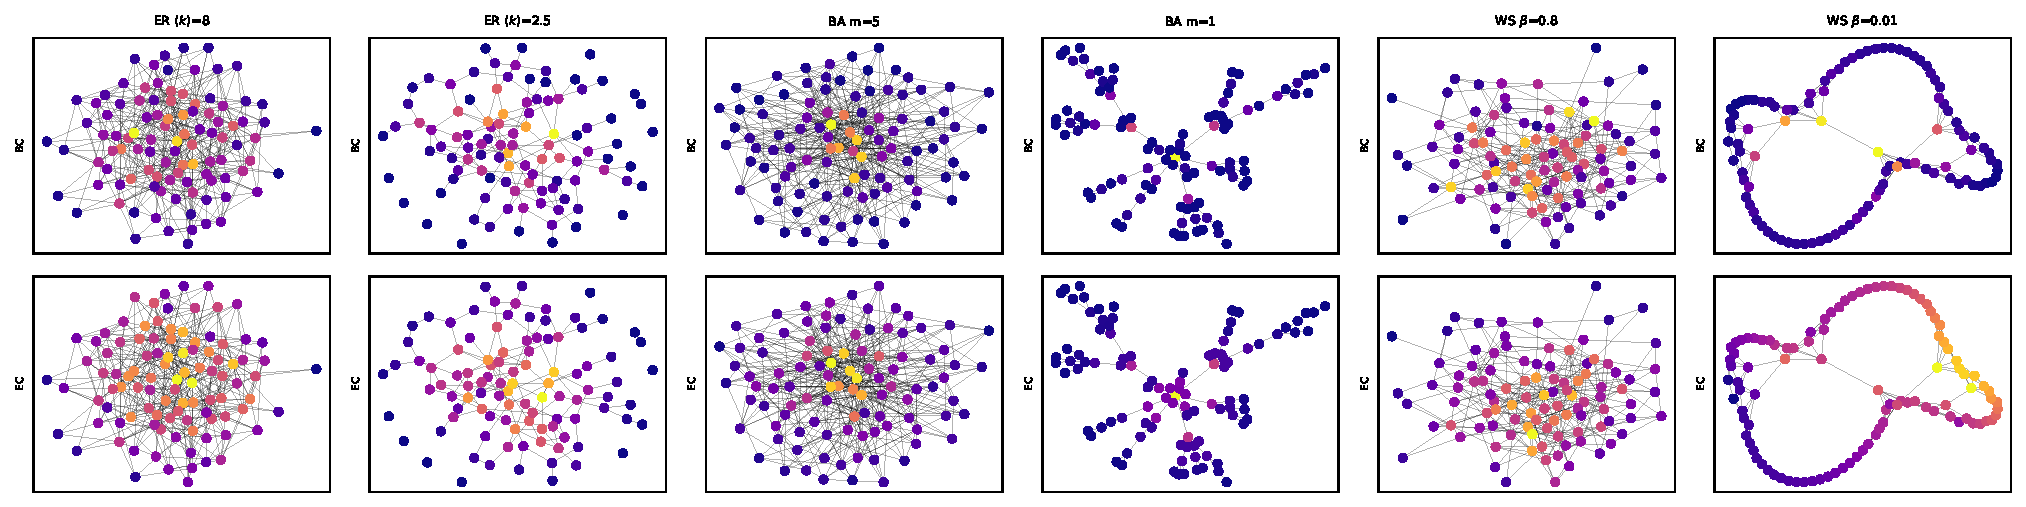
\includegraphics[width=\columnwidth]{fig1_network_viz}
  \caption{Network visualizations for high- and low-connectivity examples of
           each model~($N=100$).
           Top row: nodes colored by BC; bottom row: by EC.
           Color scale: plasma, normalized per panel.
           At low connectivity~(ER $\langle k\rangle=2.5$, BA $m=1$,
           WS $\beta=0.01$), BC identifies bridge and hub nodes that EC fails
           to differentiate.}
  \label{fig:network_viz}
\end{figure}

\begin{figure}[t]
  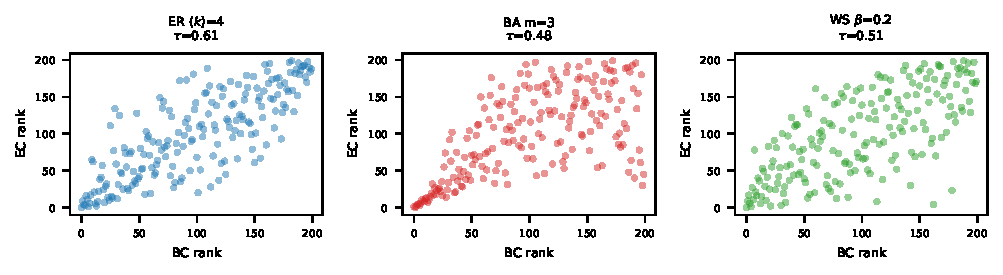
\includegraphics[width=\columnwidth]{fig2_rank_scatter}
  \caption{BC rank vs.\ EC rank for representative intact networks~($N=200$),
           annotated with Kendall~$\tau$.
           Correlation is high for ER and BA but lower for WS~($\beta=0.2$)
           where degree homogeneity compresses EC scores.}
  \label{fig:rank_scatter}
\end{figure}

\begin{figure*}[t]
  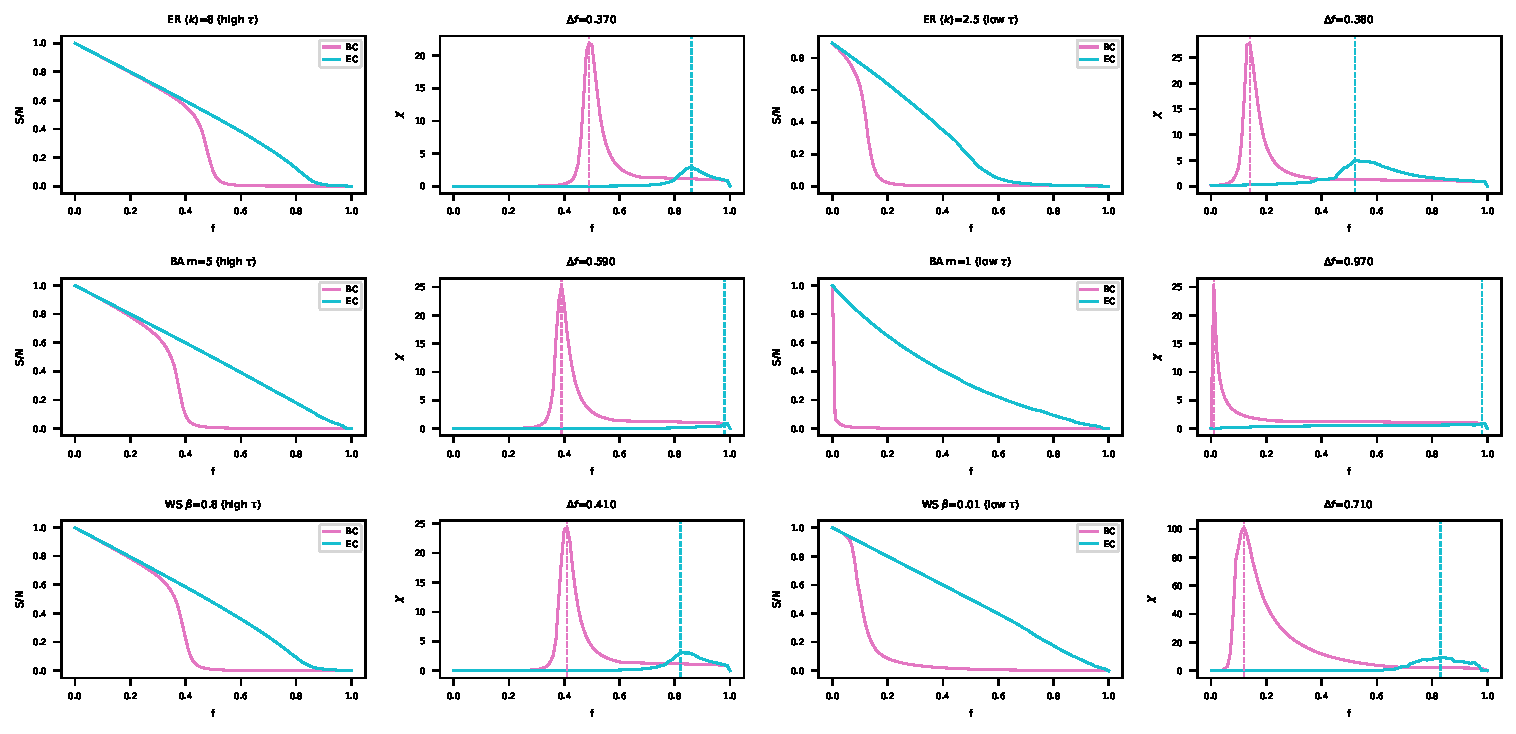
\includegraphics[width=\textwidth]{fig3_attack_curves}
  \caption{Attack curves $S(f)$ (giant fraction) and $\chi(f)$ (susceptibility)
           for BC (pink) and EC (cyan) attackers at $N=1000$.
           Left pair per model: high connectivity~(high $\tau$);
           right pair: low connectivity~(low $\tau$, where EC degrades).
           Dashed verticals mark $f_c$; $\Delta f$ is annotated in
           susceptibility panels.
           BC curves collapse earlier in all conditions.}
  \label{fig:attack_curves}
\end{figure*}

\begin{figure}[t]
  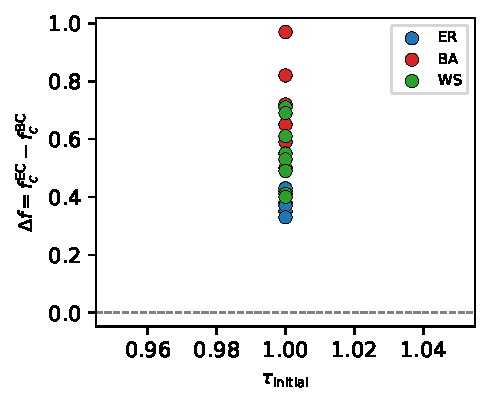
\includegraphics[width=\columnwidth]{fig4_main_scatter}
  \caption{$\Delta f$ vs.\ initial Kendall $\tau_{\rm initial}$ for all
           23 conditions at $N=1000$, colored by model.
           All points cluster near $\tau=1$ regardless of model or parameter,
           yet $\Delta f$ spans $[0.33,0.97]$.
           Initial rank agreement does not predict attack effectiveness gap.
           Dashed line: $\Delta f=0$.}
  \label{fig:main_scatter}
\end{figure}

\begin{figure}[t]
  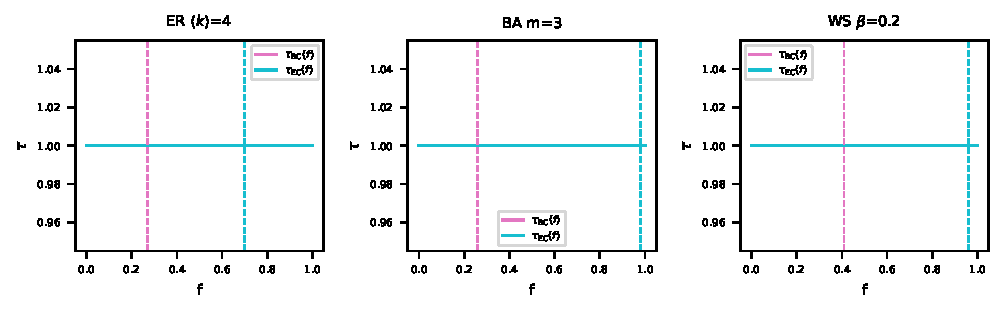
\includegraphics[width=\columnwidth]{fig5_tau_trajectories}
  \caption{$\tau$ between BC and EC rankings on the residual graph, measured
           during BC attack (pink) and EC attack (cyan), as a function of
           removal fraction $f$.
           Both trajectories remain near $\tau=1$ throughout, confirming that
           rank agreement is maintained during the attack.
           Dashed verticals mark $f_c^{\rm BC}$ and $f_c^{\rm EC}$.}
  \label{fig:tau_traj}
\end{figure}

\begin{figure}[t]
  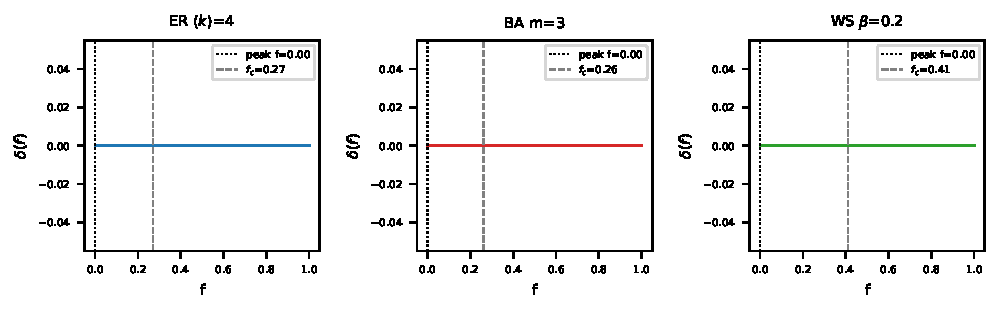
\includegraphics[width=\columnwidth]{fig6_tau_div_rate}
  \caption{$\tau$ divergence rate
           $\delta(f)=d[\tau_{\rm BC}(f)-\tau_{\rm EC}(f)]/df$
           per model.
           Near-zero values throughout confirm that the two attack trajectories
           maintain similar Kendall $\tau$ profiles;
           the gap $\Delta f$ does not arise from rank divergence during the
           attack.
           Dotted: peak of $|\delta|$; dashed: $f_c^{(\rm first)}$.}
  \label{fig:tau_rate}
\end{figure}

\begin{figure}[t]
  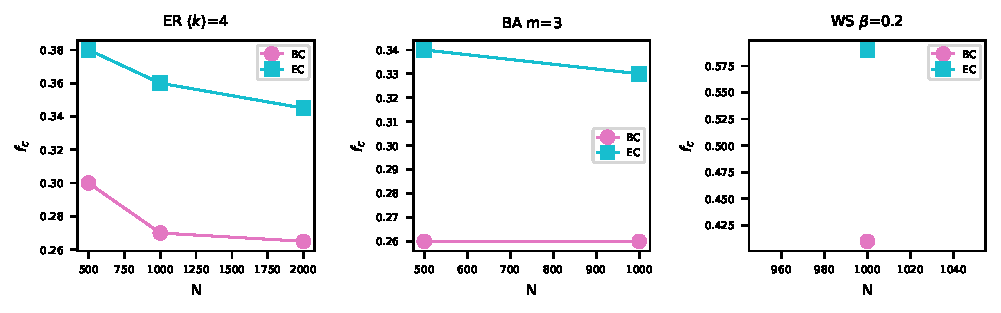
\includegraphics[width=\columnwidth]{fig7_fss}
  \caption{Finite-size scaling: $f_c$ vs.\ $N\in\{500,1000,2000\}$ for
           BC-attacker~(circles) and EC-attacker~(squares) at mid-connectivity
           conditions~(ER $\langle k\rangle=4$, BA $m=3$, WS $\beta=0.2$).
           All estimates vary by less than $\pm 0.03$ across system sizes,
           validating $N=1000$ as sufficient.}
  \label{fig:fss}
\end{figure}

% ── References ────────────────────────────────────────────────────────────────
\begin{thebibliography}{1}

\bibitem{Albert2000}
R.~Albert, H.~Jeong, and A.-L.~Barab\'asi,
``Error and attack tolerance of complex networks,''
\textit{Nature}, vol.~406, pp.~378--382, 2000.

\bibitem{Holme2002}
P.~Holme, B.~J.~Kim, C.~N.~Yoon, and S.~K.~Han,
``Attack vulnerability of complex networks,''
\textit{Phys.\ Rev.\ E}, vol.~65, p.~056109, 2002.

\bibitem{Iyer2013}
S.~Iyer, T.~Killingback, B.~Sundaram, and Z.~Wang,
``Attack robustness and centrality of complex networks,''
\textit{PLOS ONE}, vol.~8, no.~4, p.~e59613, 2013.

\bibitem{MolloyReed1995}
M.~Molloy and B.~Reed,
``A critical point for random graphs with a given degree sequence,''
\textit{Random Struct.\ Algorithms}, vol.~6, no.~2--3, pp.~161--179, 1995.

\bibitem{Barabasi1999}
A.-L.~Barab\'asi and R.~Albert,
``Emergence of scaling in random networks,''
\textit{Science}, vol.~286, no.~5439, pp.~509--512, 1999.

\bibitem{Watts1998}
D.~J.~Watts and S.~H.~Strogatz,
``Collective dynamics of small-world networks,''
\textit{Nature}, vol.~393, pp.~440--442, 1998.

\end{thebibliography}

\end{document}
